\documentclass{beamer}

\usepackage[utf8]{inputenc}
\usepackage{eurosym}
\usepackage{hyperref}
\hypersetup{
    colorlinks = true
    }
\usepackage{graphicx}
\usepackage{verbatim}

%Information to be included in the title page:
\title{GTA Einführung Robotik mit Makecode}
\author{Mattias Schlenker}
\institute{Wilhelm-Ostwald-Gymnasium}
\date{25. Februar 2021}

\begin{document}

\frame{\titlepage}

\begin{frame}
\frametitle{Viele, viele Essensrationen}
 
In dieser Stunde wollen wir unsere Map um Essenrationen oder Münzen erweitern, die Punkte oder zusätzliche Leben geben. Realisiert werden soll das mit Sprites, die ihre Position behalten:

 \begin{figure}
  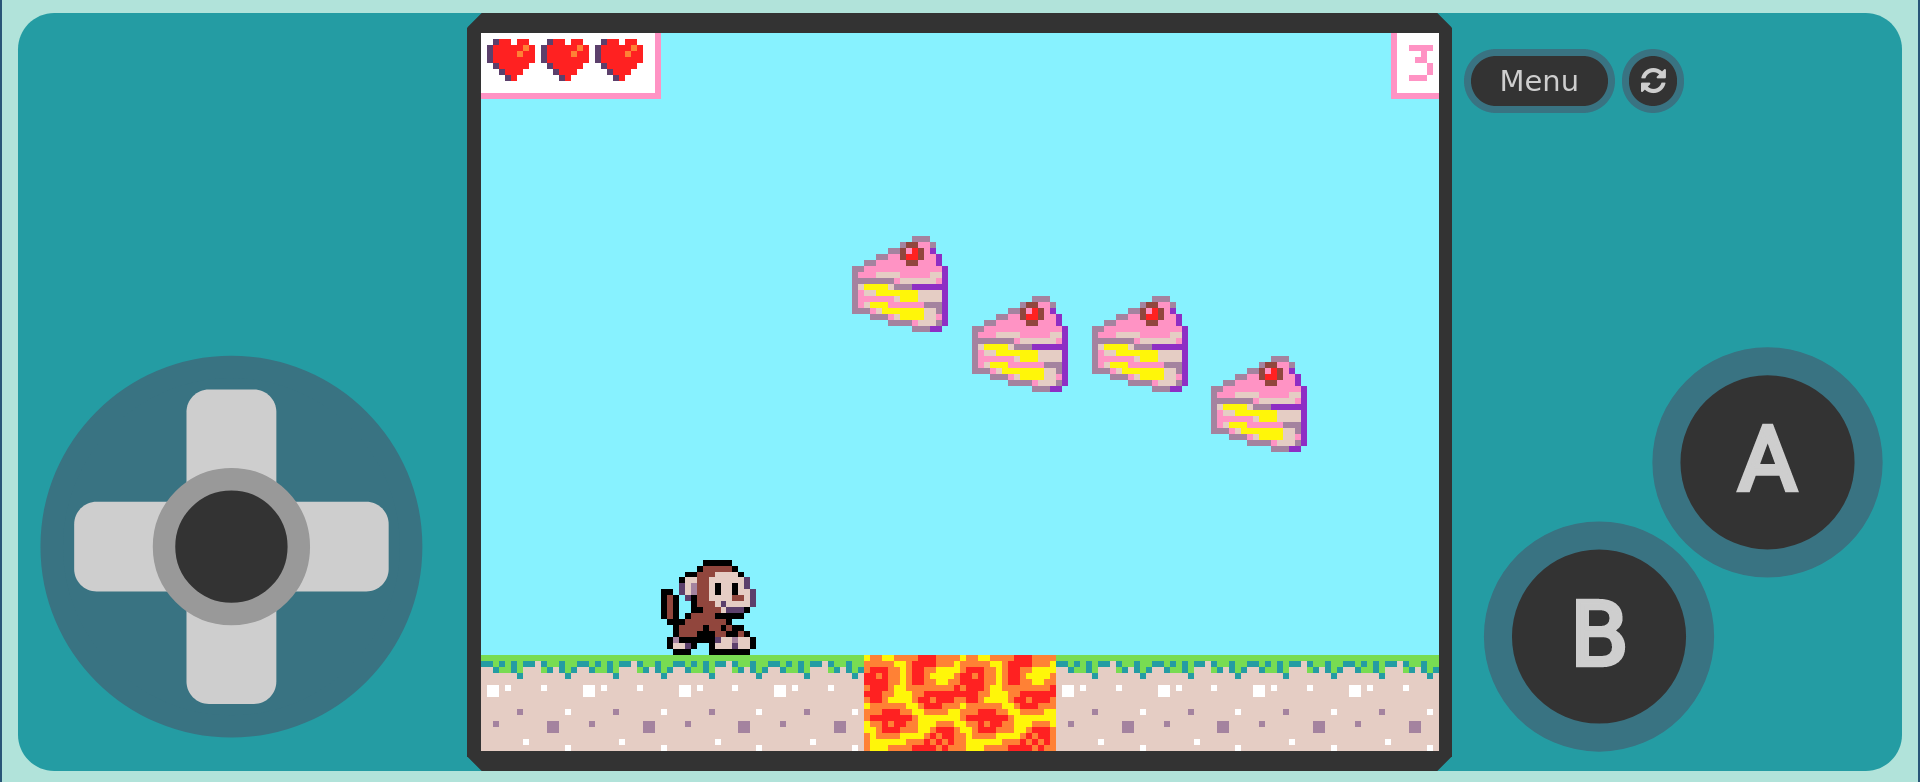
\includegraphics[width=8cm]{game38.png}
  \caption{Kuchenstücke}
  \label{fig:game38}
\end{figure}

Wie realisieren wir das ohne jeden Sprite von Hand zu positionieren? 

\end{frame}

\begin{frame}
 \frametitle{Arrays oder Listen}
 
Die verwendete Datenstruktur nennt sich Liste oder Array, Ihr kennt sie vom Einkaufen:

\begin{itemize}
\item Milch
\item Kartoffeln
\item Nuss-Nougat-Creme
\item Rosenkohl
\end{itemize}

Beim Einkaufen nehmt Ihr immer ein Element von der Liste, packt es in den Einkaufswagen und streicht es ab.
 
\end{frame}

\begin{frame}[fragile]
 \frametitle{Listen in der Informatik}
 
In Pseudocode schreibt Ihr Listen Komma getrennt in eckigen Klammern. Unsere Liste für die x-Koordinaten der Essensrationen könnte also so aussehen:

\begin{verbatim}xPositionenKuchen = [ 30, 50, 70, 110, 130, 150 ] \end{verbatim}
 
\end{frame}

\begin{frame}
\frametitle{Vorarbeit in Makecode}

Um besser arbeiten zu können, setzt zunächst im Spielupdate-Block die Wahrscheinlichkeit für Haie auf 0\%. Dann soll der Affe anhalten, wenn das Steuerkreuz nicht mehr gedrückt wird. Dafür wird das Controller-Event ,,Taste losgelassen'' benutzt:

 \begin{figure}
  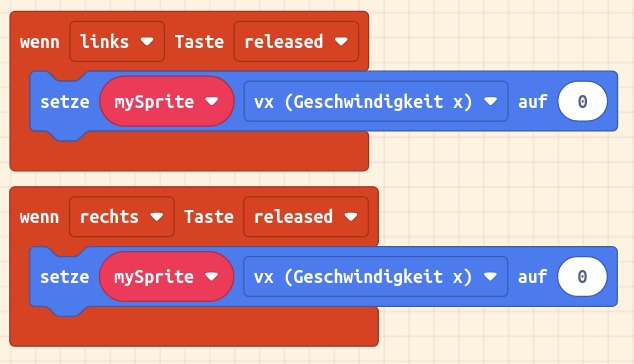
\includegraphics[width=6cm]{game39.png}
  \caption{Controller-Events}
  \label{fig:game39}
\end{figure}

\end{frame}

\begin{frame}
 \frametitle{Listen in MakeCode}
 
Klappt in der Kategorieübersicht ,,Fortgeschritten'' auf und sucht in ,,Arrays'' nach dem Block, der einer Variable ein Array/eine Liste  zuweist. Diese Liste hat zunächst zwei Elemente. Gebt der Variablen den Namen ,,xPositionenKuchen'' und tragt die ersten beiden Werte der Liste von der vorletzten Folie ein. 

  \begin{figure}
  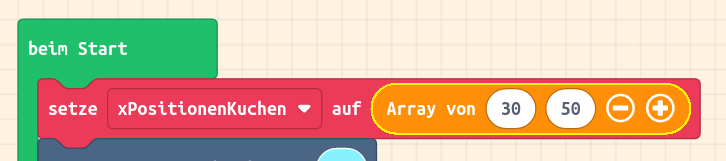
\includegraphics[width=8cm]{game40.png}
  \caption{Liste mit zwei Elementen}
  \label{fig:game40}
\end{figure}

 
\end{frame}

\begin{frame}
 \frametitle{Liste erweitern}
 
Verwendet den Plus-Knopf, um diese Liste zu erweitern. Tragt für Eure Map sinnvolle Werte ein. Denkt daran, dass eine Kachel und unsere Standard-Sprites je 16 Pixel Seitenlänge haben:

\begin{figure}
  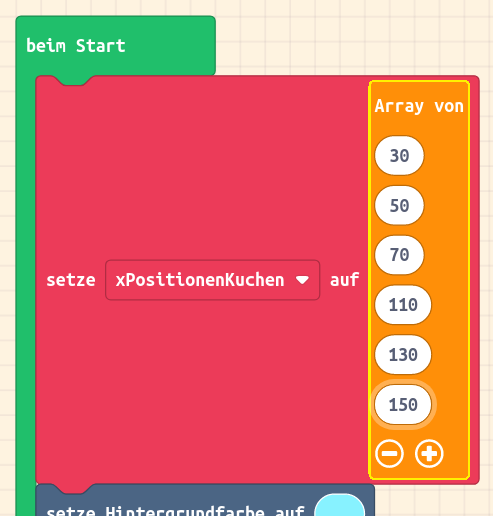
\includegraphics[width=5cm]{game41.png}
  \caption{Liste wird länger}
  \label{fig:game41}
\end{figure}
\end{frame}

\begin{frame}
 \frametitle{Array-Operationen}
 
\textbf{Achtung:} Hier arbeiten wir mit Listen variabler Länge, fragt in Microcontroller- oder Robitik-Projekten Eure Dozenten, ob Listen in der verwendeten Programmierumgebung feste oder variable Längen haben!

Wichtige Array-Operationen sind:

\begin{itemize}
\item Rufe ein durch einen Index angegebenes Element ab (bspw. das dritte hat Index 2)
\item Nehme den ersten Wert der Liste (Liste wird kürzer)
\item Nehme den letzten Wert der Liste (Liste wird kürzer)
\item Füge am Anfang oder Ende ein Element an
\end{itemize}
 
Mit den letzten drei Operationen kann man eine Liste wie eine Warteschlange (vorne wegnehmen und hinten anhängen) oder einen Stapel (was zuletzt draufgelegt wurde, wird als erstes weggenommen) behandeln.
 
\end{frame}

\begin{frame}
 \frametitle{Kuchen platzieren 1}
 
Nun bietet es sich an, solange X-Koordinaten von der Liste wegzunehmen, bis die Liste leer ist und erst dann zum nächsten Block zu gehen. Wir fügen also einen Block ,,während'' ein, der aus Logik einen Vergleichsoperator ,,größer'' mitbekommt:

\begin{figure}
  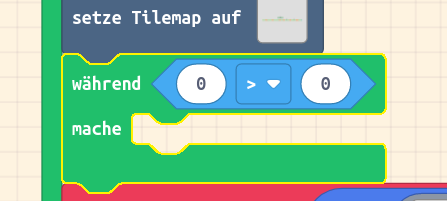
\includegraphics[width=8cm]{game42.png}
  \caption{Vorbereitung der Prüfung auf Listenlänge}
  \label{fig:game42}
\end{figure}

\end{frame}


\begin{frame}
 \frametitle{Kuchen platzieren 2}
 
An die erste Stelle des Vergleichsoperators setzen wir nun die Länge des Arrays ,,xPositionenKuchen'': 

\begin{figure}
  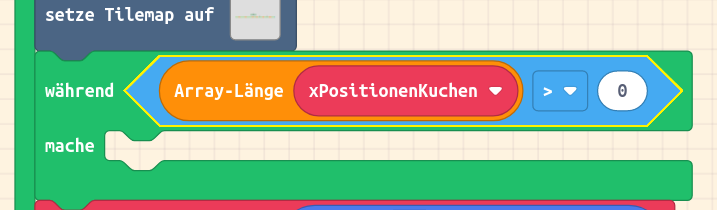
\includegraphics[width=8cm]{game43.png}
  \caption{Prüfung auf Listenlänge – sind noch Werte in der Liste?}
  \label{fig:game43}
\end{figure}

Da die Liste nie kürzer wird, bleibt Euer Bildschirm schwarz, wenn Ihr das Spiel jetzt startet…

\end{frame}

\begin{frame}
 \frametitle{Kuchen platzieren 3}
 
Jetzt kommt ein Sprite der Art ,,Food'' ins Spiel. Als X-Position bekommt er den ersten Wert der Liste ,,xPositionenKuchen'', die Y-Position weit genug vom oberen Rand, damit der Kuchen durch Hüpfen erreichbar ist . Die Liste wird dadurch in jedem Durchgang kürzer. Ist die Länge 0, wird der nächste Block angesprungen: 
 
\begin{figure}
  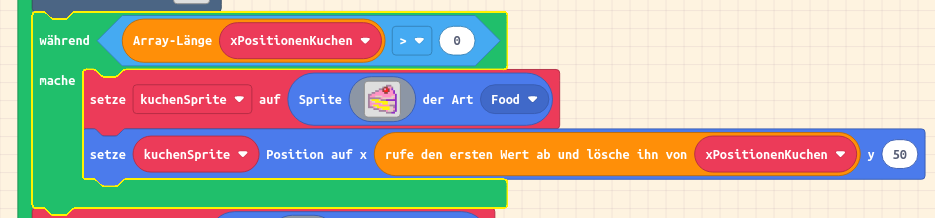
\includegraphics[width=10cm]{game44.png}
  \caption{Liste verkürzen}
  \label{fig:game44}
\end{figure}
\end{frame}

\begin{frame}
 \frametitle{Hmmmm…}
 
 Alle Kuchen auf derselben Höhe? Das ist doch langweilig oder? Klar, wir hatten immer den gleichen Y-Wert…
 
\begin{figure}
  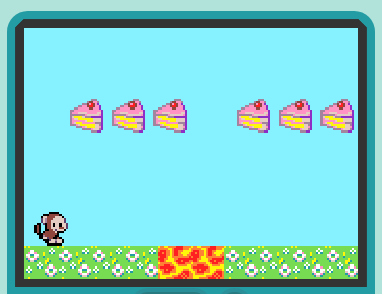
\includegraphics[width=7cm]{game45.png}
  \caption{Kuchenhöhe in eigener Liste}
  \label{fig:game45}
\end{figure}
\end{frame}

\begin{frame}
 \frametitle{Liste für die Y-Werte}
 
OK, erstellen wir durch Kopieren und umbenennen eine Liste ,,yPositionenKuchen'' in der wir die Höhe zwischen 80 und 60 Pixeln vom oberen Rand variieren:
 
\begin{figure}
  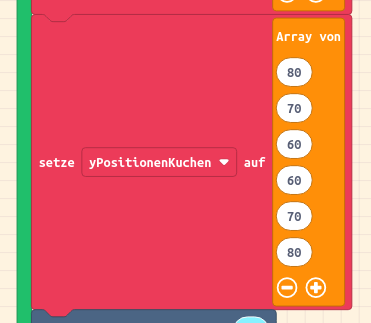
\includegraphics[width=6cm]{game46.png}
  \caption{Kuchenhöhe als Liste}
  \label{fig:game46}
\end{figure}
\end{frame}


\begin{frame}
 \frametitle{Y-Werte aus Liste entnehmen}
 
Für die Y-Koordinate kopieren wir den Block ,,rufe den ersten Wert ab und lösche ihn von xPositionenKuchen'' und benennen die Variable um in ,,yPositionenKuchen''. Dann schieben wir ihn an die Stelle der bisher fixen Höhe:
 
\begin{figure}
  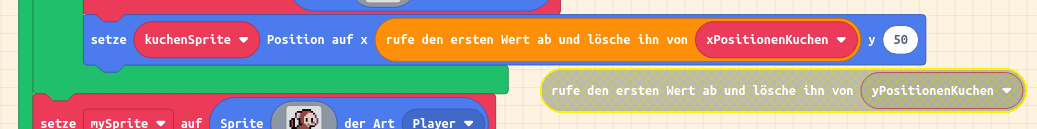
\includegraphics[width=10cm]{game47.png}
  \caption{Kopiert und umbenannt…}
  \label{fig:game47}
\end{figure}
\begin{figure}
  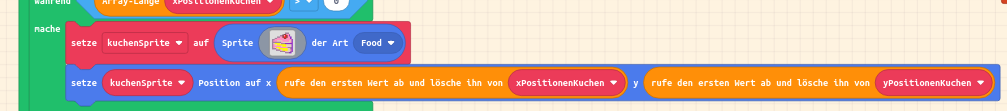
\includegraphics[width=10cm]{game48.png}
  \caption{…und an der richtigen Stelle eingefügt}
  \label{fig:game48}
\end{figure}

\end{frame}

\begin{frame}
 \frametitle{Kollisionserkennung}
 
Die Kollisionserkennung funktioniert wie beim Shooter. Nichts neues hier. Vergesst nicht, im Start-Block die Punktzahl auf 0 zu setzen:
 
\begin{figure}
  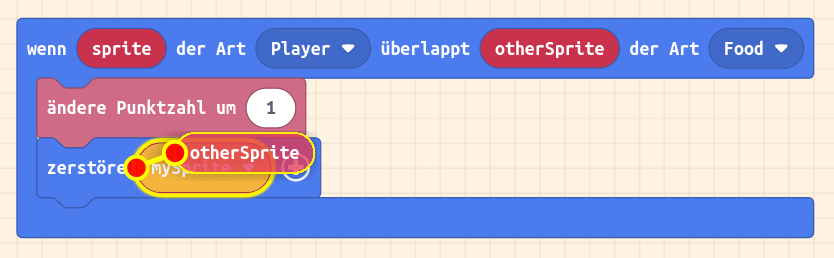
\includegraphics[width=10cm]{game49.png}
  \caption{Zerstören des Food-Sprites und Inkrementieren der Punkte}
  \label{fig:game49}
\end{figure}
\end{frame}
 

\begin{frame}
 \frametitle{Download des Musterspiels}

Wie die letzten Termine steht die UF2-Datei in LernSax, alternativ könnt Ihr hier direkt weitermachen:

\href{https://makecode.com/\_Jjh8rqMsa8y0}{https://makecode.com/\_Jjh8rqMsa8y0} 

Wer arbeitet an einer spannenderen Map mit mehr Essenrationen und vielleicht Zusatzleben nach Kontakt mit einem Gegner?

In den nächsten Sessions arbeiten wir weiter an den eingereichten Vorschlägen.
\end{frame}

\end{document}
